\documentclass[11pt, oneside]{article}
\usepackage[margin=1in]{geometry}
\geometry{letterpaper}
\usepackage{booktabs}
\usepackage{hyperref}
\usepackage{enumitem}
\usepackage{float}
\usepackage{caption}
\usepackage[numbers]{natbib}
\usepackage{graphicx}
\usepackage{amsmath}
\usepackage{amssymb}
\usepackage{array}
\usepackage{xcolor}
\usepackage{adjustbox}

\hypersetup{colorlinks=true, linkcolor=blue, citecolor=blue, urlcolor=blue}
\graphicspath{{figures/}}
\captionsetup{font=small}
\setlength{\textfloatsep}{8pt}
\setlength{\floatsep}{6pt}
\setlength{\intextsep}{6pt}
\newcommand{\run}[1]{\texttt{#1}}
\newcommand{\hyp}{\textsc{hypothesis}}

\title{Data Analysis\\[2pt]
\large CS781 Capstone: In-House Legal Intelligence System}
\author{Sanskaar Srivastava (220967)\\}
\date{}

\begin{document}
\maketitle



\section{How this analysis was done}
\textbf{Inputs.} The official data files of all seven phases; the logs, validation metrics and saved scores of every
training run; the outputs of the offline post-processing scripts; and the Codabench scores the student reported.
No hidden test label was used, and no setting was chosen here.

\textbf{Order of evidence.} Results were weighed in this order: (1) controlled comparisons that change one factor on
the same split; (2) 2-fold cross-validated (CV) estimates of decisions fitted on validation data; (3) single validation
scores; (4) Codabench scores. Codabench scores are used only to judge how well local estimates predicted the test set,
never to rank alternatives.

\textbf{How large a difference must be.} The validation sets differ in size by three orders of magnitude, so the same
difference means different things in different phases. Phase~4 has 994 balanced development cases: for an
accuracy-like score near 0.75 the sampling standard error is $\sqrt{0.75\cdot0.25/994}\approx0.014$. Phases~2 and~3
validate on 10 documents and Phase~7 on 118 queries, where whole documents or queries move together, so the
uncertainty is larger than the sentence or span counts suggest. For Phase~7 the 20 repeated CV splits vary with a
standard deviation of only 0.0024, but that measures how the split changes the result, not sampling error. In practice,
differences below about 0.01 in Phases~2, 3 and~7 were not treated as real unless the same direction appeared across
several runs or models.

\textbf{How a conclusion was reached.} For each result I looked for a mechanism, then for a second, independent
observation that the mechanism also predicts. An example is the Phase~3 gap between development and Codabench
(Section~\ref{sec:calib}): the explanation (two roles missing from development) predicts a specific rescaling factor,
and that factor removes most of the gap.

\section{What the data says}\label{sec:data}
\textbf{Phase 1: an under-trained regime by construction.} The Supreme Court file holds about 275M tokens, and one
epoch for a 101M model is about two tokens per parameter, roughly a tenth of what is usually compute-optimal. The test
prompts are closest to Supreme Court text (tokenizer fertility 1.070 against 1.085 for a uniform mix of all four
domains), so adding High Court and Tribunal text was not free: it would buy data at the cost of domain match. Every
later observation should be read with this in mind. The backbones are data-starved, which favours methods that extract
more from fixed data and decisions that exploit dataset statistics.

\textbf{Phase 2: labels defined by form are easy; labels defined by role are hard.} Dates (1{,}575 training spans),
statutes (1{,}260) and precedents (1{,}183) have a recognisable surface form. Appellant (407), respondent (381),
appellant's counsel (195), respondent's counsel (184) and witness (187) are all \emph{person names}, distinguished
only by the role the person plays in the case. The per-label results largely follow this split. The best run reaches
0.93 F1 on dates, 0.85 on statutes and 0.79 on courts, but only 0.11 on appellants, 0.21 on respondents, 0.24 on
appellant's counsel and 0.22 on witnesses (respondent's counsel, 0.46, is the exception). Rarity alone does not explain
it: judges (245 spans) are also rare but carry a strong form cue (``J.'', ``Justice'') and reach 0.76. \hyp: the role cue usually lies in the header (``\ldots Appellant'') or far from a later
mention, beyond the window, so the model sees a name without its role. The data supports the first half: first party
mentions lie within 256 tokens in 98\%/94\% of documents, while half of all mentions lie beyond token 1{,}024. The
second constraint is the metric. Only 60\% of gold spans end on a word boundary, so without the trimming rules the
pipeline could not exceed 0.605 strict macro-F1 even with perfect tags (0.979 with them). Getting offsets right was
a precondition, not a refinement.

\textbf{Phase 3: the same form/role pattern at sentence level.} The largest confusions are \emph{ArgumentPetitioner}
predicted as \emph{ArgumentRespondent} (136 development sentences) and \emph{Fact} predicted as
\emph{RatioOfTheDecision} (75). Arguments from the two sides have the same form and differ only in who makes them.
Facts and reasoning both narrate the case and differ in function. The domains differ (Corporate Law has \emph{Dissent},
284 training sentences; IT has more \emph{Statute} and \emph{None}), and Corporate Law is harder in all 17 runs. Two
roles never occur in development, which caps any development macro-F1 at $11/13=0.846$ and, as shown in
Section~\ref{sec:calib}, distorts every development-to-test comparison.

\begin{figure}[H]
\centering
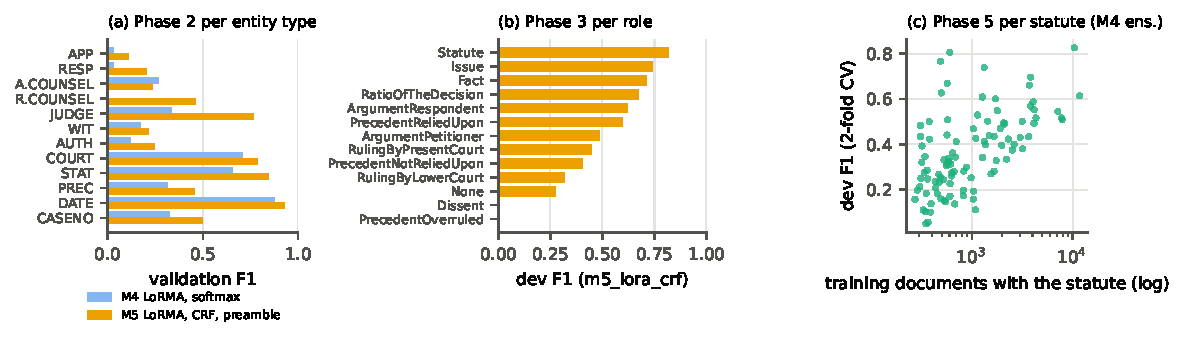
\includegraphics[width=\textwidth]{per_class.pdf}
\caption{Per-class results (from the report): (a) Phase~2 F1 per entity type, first and best system; (b) Phase~3 F1 per
role; (c) Phase~5 F1 per statute against its training frequency.}
\label{fig:perclass}
\end{figure}

\textbf{Phase 4: a prior shift and less explicit test cases.} Training is 41.4\% positive, development 50\%.
Macro-F1 weighs both classes equally, so a model calibrated to the training prior under-predicts acceptances on
development, which the runs did. Explicit outcome words (allowed/dismissed) occur in 24\% of training tails but only
13\% of test tails. The organisers seem to have removed the outcome statement more thoroughly from the test cases,
so a model that learned to read the verdict sentence is penalised on test. The leaked test labels inside
\texttt{dev.json} (all 1{,}517 test cases) made it essential to validate only on the 994 other cases.

\textbf{Phase 5: a long tail that the metric weighs equally.} Statutes range from 11{,}731 to 272 training
documents, and macro-F1 gives each statute the same weight. Per-statute F1 rises with training frequency (Spearman
$\rho=0.57$): mean F1 is 0.25 in the rarest quarter, 0.35 and 0.37 in the middle quarters and 0.51 in the most frequent
quarter. The 57 statutes with fewer than 1{,}000 training documents average 0.29, the five with more than 5{,}000
average 0.60. Statute names are masked in the text, so the model must infer the statute from the facts. Thresholds
tuned for macro-F1 trade precision for recall on rare labels: the system predicts 5.2 statutes per development
document against 3.9 gold.

\textbf{Phase 6: the metric reads only the opening of the summary.} Documents have a median of 3{,}146 words and
summaries 641 (compression 4.6). 79\% of summary bigrams occur in the document, so the references are close to
extractive. The models read 1{,}024 document tokens (head and tail), roughly a quarter of a median document. The
official BERTScore model truncates both texts at about 512 of its own tokens, so only the first $\approx$400 words of
a summary are compared. A summary's later content, which carries the decision, is invisible to the primary metric.
This explains why very different systems land within a few thousandths of each other (Section~\ref{sec:results}).

\textbf{Phase 7: the exactly-seven rule caps the score.} A query has 6.4 relevant cases on average in training
(median 4) and 8.2 in development (median 5). 59\% of development queries have fewer than seven relevant cases and
33\% have more, so returning exactly seven guarantees false positives for most queries and misses for many others. A
perfect ranker would score at most 0.618 Micro-F1@7 on development (0.639 on training). The best development
estimate, 0.433, is therefore about 70\% of the reachable score, not 43\%. Three structural facts matter more than any text property: a query is in
its own pool but never its own answer; relevant cases are earlier; and each candidate is relevant to about one query.
The last fact turns the problem into something close to an assignment. A candidate that scores well for \emph{every}
query (long, generic, citing many statutes) is unlikely to be the answer to any particular one. Finally, the header
field \emph{CITATOR INFO} lists the later cases citing a judgment and matched the query in 105 of 214 sampled relevant
pairs, a label leak that was removed before any modelling.

\section{What moved the metric in each phase}\label{sec:results}
Table~\ref{tab:levers} sets the largest gain from the backbone or training next to the largest gain from the decision
layer (everything computed after the network) for each phase.

\begin{table}[H]
\centering\small
\caption{The largest training-side lever and the largest decision-side lever per phase (one factor changed;
validation or CV unless marked LB = Codabench).}
\label{tab:levers}
\begin{adjustbox}{max width=\textwidth}
\begin{tabular}{c>{\raggedright\arraybackslash}p{6.4cm}>{\raggedright\arraybackslash}p{6.6cm}}
\toprule
Phase & Backbone / training lever & Decision-layer lever\\
\midrule
1 & M1 $\to$ M4 (architecture, recipe, tokens): +0.049 LB & repetition control and penalty: +0.004 LB; MBR consensus: a further +0.004 LB (+0.037 over plain greedy, pseudo-val.)\\
2 & M4 $\to$ M5 backbone (LoRMA, CRF, preamble): +0.024 & softmax $\to$ CRF: +0.130; document rules on the CRF: +0.031\\
3 & best M2 $\to$ best M5 submission: +0.076 LB & own CRF $\to$ prior + training-transition Viterbi (\run{m5\_crf\_ens}): +0.067 LB\\
4 & 10k $\to$ 31.7k training cases: +0.029 to +0.058 & 8-chunk test reading + dev threshold (\run{m5\_rslora\_alldocs}): +0.045 (CV)\\
5 & full vs.\ LoRMA fine-tuning (M5): +0.024 & per-statute vs.\ global thresholds: +0.013 (CV)\\
6 & M3 GRU $\to$ M4 decoder: +0.035 held-out & repetition penalty 1.15: +0.005 held-out\\
7 & fine-tuning M5 LoRMA from Phase~1 weights: +0.067 raw & BM25 fusion, normalisation, rules: +0.122 (0.3091 $\to$ 0.4308 CV)\\
\bottomrule
\end{tabular}
\end{adjustbox}
\end{table}

\textbf{Phase 1.} The architecture sequence gave the largest gain (0.7830 $\to$ 0.8324). This cannot be divided among
RoPE, GQA, RMSNorm and SwiGLU, because each step also changed size, batch or tokens seen; what it shows is that the
recipe made a full epoch possible. Among decoding settings, repetition control decided the outcome. Plain greedy decoding repeats 69\% of
its word 4-grams, and a 3-gram block alone adds 0.030 BERTScore. Longer blocks are worse (a 6-gram block lets 17\% of
4-grams repeat because the model rephrases around the ban). The penalty raises BERTScore but lowers ROUGE-L
(0.1995 $\to$ 0.1865), and beam search gives the best ROUGE-L and BLEU but a middling BERTScore. The two metrics reward
different things: BERTScore rewards bringing in new legal content, word overlap rewards safe, generic phrasing. MBR
selection was the strongest setting on pseudo-validation (+0.0047) and, submitted, gave the best Phase~1 result:
0.8407 on Codabench, 0.0012 below its pseudo-validation score and +0.0044 over the best single decoding setting.

\textbf{Phase 2.} The output layer mattered most. A CRF raised validation strict macro-F1 from 0.3202 to 0.4502, while
constrained Viterbi on the same softmax scores reached 0.4131. About 70\% of the gain therefore comes from only
decoding valid tag sequences, and the remaining 30\% from training on whole sequences with learned transitions. The document rules show a clean mechanism. Propagation
copies every predicted string to its other occurrences, so it multiplies the base system's precision: it added 0.024
to the CRF (precision 0.531), cost 0.007 with constrained Viterbi (0.422) and cost 0.020 with fully fine-tuned softmax
(0.335). Propagation is worth applying only on top of a high-precision tagger. The 256-token preamble added 0.006, which
is within the noise of 10 documents, though it is consistent with where the parties are named. The greedy span ensemble
looked best on validation and failed on test because its selection reused the same 10 documents.

\textbf{Phase 3.} Decoding with training-label statistics was the strongest single lever on test. Logit adjustment by
the training role prior pushes predictions toward rare roles, which macro-F1 rewards. The training transition matrix
enforces the order of a judgment. On \run{m5\_crf\_ens} this moved Codabench from 0.504 to 0.571, more than the
learned CRF transitions did. Ensembling four runs of one model was the second lever (0.571 vs.\ 0.543 for the best
single CRF run with the same decoding). The position prior raised development F1 but lowered Codabench F1 for the
ensembles (\run{m5\_crf\_ens}: 0.571 $\to$ 0.556), while it helped one single run (0.543 $\to$ 0.559). It is computed
from training data, so this is not overfitting by selection. With 10 development documents, its effect is within the
noise in either direction.

\textbf{Phase 4.} Three levers stand out. First, \emph{what to read}: models trained on the last 512 tokens score
0.62--0.66 when reading the tail but 0.53--0.57 reading the head, matching where judgments state their outcome.
Second, \emph{how much data}: training on all 31.7k cases instead of 10k added 0.029--0.058 across the four M5
methods. Third, \emph{the decision threshold}: fitting it on development data corrects the prior shift (41\% vs.\
50\%). A useful near-controlled comparison: for LoRMA, tripling the data (0.6233 $\to$ 0.6519, 175 minutes) and
quadrupling the reading length (0.6566, 192 minutes) cost about the same and gained about the same. The best submission
combines all three levers (0.7609).

\textbf{Phase 5.} Full fine-tuning beat LoRMA on both decoders (M4 0.3535 vs.\ 0.3414; M5 0.3531 vs.\ 0.3292), the
clearest gap between full and parameter-efficient training in the project. \hyp: 100 independent decision
boundaries, many for rare labels, need more change to the representation than a near-identity re-mixing of the
frozen layers provides, at least at the shared, untuned adapter learning rate. More data again beat longer reading:
LoRMA on all 42k documents reading one chunk (0.3490) beat LoRMA on 15k documents reading four (0.3292). Per-statute
thresholds added 0.013 over one global threshold, the expected direction for a long tail.

\textbf{Phase 6.} The three decoders are within 0.002 held-out BERTScore (M4 LoRA 0.8378, M2 Houlsby 0.8377,
M5 LoRMA 0.8361), although their ROUGE scores and summary lengths differ (535 to 664 words). This compression of
differences is what the truncation in Section~\ref{sec:data} predicts. Only the GRU (0.8033, stopped at 0.94 epochs by
its time budget) and the 4-layer student (0.8232) are clearly separated. Generated summaries are shorter than the
references (535 vs.\ 852 words on average), and 11\% hit the length cap. Reading the tail as well as the head added
0.0024, consistent with the decision being stated at the end of the judgment.

\textbf{Phase 7.} Post-processing dominated. Every system, including BM25 with no learning, lands between 0.425 and
0.433 CV after the same post-processing. Fine-tuning lifts the raw dense ranking of the 10-layer decoders from 0.24 to
0.31 (0.34 when reading four chunks), but that gain almost disappears once the scores are fused and normalised. The key
step is column normalisation: z-scoring each candidate's scores across all queries. BM25 with the rules but without
column normalisation scores 0.188 on development; with it, 0.426 (CV).
This is the assignment structure from Section~\ref{sec:data}. Removing each candidate's general ``popularity'' leaves
only its \emph{relative} affinity to each query, a correction for hub candidates. Once that correction is applied, a
lexical score and a dense score carry nearly the same information at this data size (827 training queries, 2$\times$512
tokens read per case). The query penalty is a bet on which split the test resembles: training (19.4\% of answers are
other queries) or development (2.0\%). On Codabench the variants without the penalty scored the same or slightly
better (0.4318 vs.\ 0.4306 for BM25), which suggests the test set resembles development.

\section{Findings across phases}\label{sec:cross}
\textbf{Which backbone transfers.} M5, the prefix-LM, gave the best submission in Phases~2, 3 and~4 and the best
model-based retrieval system in Phase~7. M4 was best as a language model (Phase~1), for summarization and for statute
identification, but in the last two by margins of 0.005 or less.
M2 was competitive when little data was used (best single 10k-case run in Phase~4, 0.6831) and in summarization. M3
was last in every phase. \hyp: M5 transfers best to reading tasks because its pretraining already used bidirectional
attention over the prompt, which is the setting all reading tasks use after the causal mask is removed. M4 had never
seen it. The evidence is consistent but not controlled: M5 was not compared with an M4 that was also given some
bidirectional pretraining.

\textbf{Parameter-efficient vs.\ full training.} With about 1\% of the parameters, LoRA and rsLoRA came within 0.02 of
full fine-tuning in Phases~3 and~4 and sometimes exceeded it (Phase~4 on all data: LoRA 0.6980, rsLoRA 0.7087, full
0.6874). rsLoRA beat LoRA in 5 of 8 paired runs, a weak preference. LoRMA was the lowest of the low-rank methods on M5
in Phases~3 and~4 and clearly below full training in Phase~5. Its best use was Phase~2, where it was the adapter
under the winning CRF system. All methods shared one untuned adapter learning rate, and LoRMA's multiplicative update
interacts with the scale of the frozen weights, so the honest conclusion is ``LoRMA under shared settings'', not
``LoRMA is worse''. IA$^3$ and BitFit, with 0.03--0.08M parameters, were clearly too small (Phase~7: 0.2690 vs.\
0.3102; Phase~2 on M3: 0.1149 vs.\ 0.1906).

\begin{figure}[H]
\centering
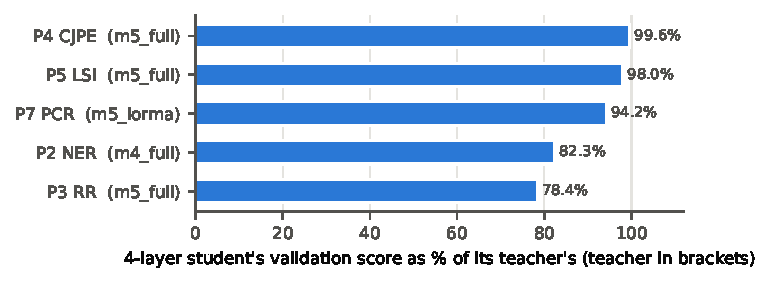
\includegraphics[width=0.62\textwidth]{llm_kd.pdf}
\caption{Knowledge distillation into a 4-layer student (63.6M parameters, $\approx$2.6$\times$ faster training).
Phase~6 is omitted because BERTScore compresses differences (student 0.8232 vs.\ teacher 0.8361).}
\label{fig:kd}
\end{figure}

\textbf{Distillation depends on the output's structure.} The 4-layer student kept 99.6\% of its teacher's score in
Phase~4 and 98.0\% in Phase~5, but only 82\% in Phase~2 and 78\% in Phase~3 (Fig.~\ref{fig:kd}). \hyp: a single
document-level label can be read from a few strong cues, which a shallow network captures. Token tags and sentence
roles depend on long-range context across a 1{,}024-token window, which needs depth. The Phase~2 control (same student
trained without a teacher: 0.2695 vs.\ 0.2841) shows that the teacher signal itself helped, not only the architecture.
In Phase~4 the student is the most cost-effective model of the project: 0.6503 in 26 minutes, against 0.6528 in 69.

\textbf{Decisions computed from data statistics were worth as much as the networks.} In Table~\ref{tab:levers} the
decision-side lever is clearly larger than the training-side lever in Phases~2 and~7 and comparable in Phases~3
and~4. Training dominates only in Phases~1, 5 and~6, where the decision layer has little structure to exploit. This is
what the under-trained regime predicts. When the backbone is limited by data, the
structure of the task (valid spans, role order, label priors, the assignment structure of retrieval) is information the
network has not learned, and adding it at decision time costs nothing in training.

\textbf{More data beat more context.} In Phase~4 (LoRMA) three times the data matched four times the reading length at
the same cost. In Phase~5 three times the data with a quarter of the reading length won by 0.020. This agrees with the
Phase~1 observation that the models are data-starved.

\section{Local estimates against Codabench}\label{sec:calib}
\begin{figure}[H]
\centering
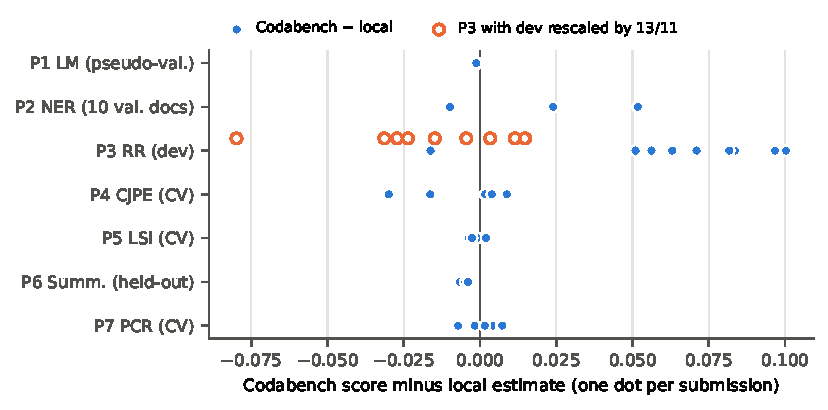
\includegraphics[width=0.78\textwidth]{llm_calibration.pdf}
\caption{Codabench score minus the local estimate for every submission whose local score was recorded.}
\label{fig:calib}
\end{figure}
Figure~\ref{fig:calib} shows how well local estimates predicted the test set. Phases~1, 5, 6 and~7 are calibrated to
within $\pm$0.008. The pseudo-validation of Phase~1 was cut from the test prompts themselves, Phase~6 held-out pairs
come from the same distribution, and Phase~7's CV covered 118 queries with 20 repeated splits. Phase~5 is the tightest:
the four submissions with a recorded CV estimate landed within 0.004 of it, including the per-statute thresholds that
were fitted on development data (0.3673 CV, 0.3664 Codabench). Phase~4 is calibrated
for the CV-based choices (within 0.017 or better), with one exception: \run{m2\_lorma} with the training-prior
threshold scored 0.7188 on development but 0.6889 on test. It was among the highest of about a hundred development
candidates, so its development score was selected for being high. This is the winner's curse, and the reason the report quotes
cross-validated estimates. Phase~2's 10 validation documents gave estimates 0.02--0.05 below test in two of three
cases, which is noise at that size.

Phase~3 is the striking case: Codabench was 0.05--0.10 \emph{above} development for nine of ten submissions. The
explanation is in the data. \emph{Dissent} and \emph{PrecedentOverruled} never occur in development, but the official
scorer averages over all 13 roles and gives an absent role F1 = 0, so development macro-F1 is the 11-role average times
$11/13$. If the test set contains these roles and the model handles them about as well as the others, test macro-F1 is
roughly development $\times\,13/11$. Rescaling turns the median gap of +0.08 into one of $-0.01$ (open circles in
Fig.~\ref{fig:calib}). The best system's gap becomes +0.015 (0.557 rescaled vs.\ 0.571). The rescaling is approximate,
but it removes most of a gap that otherwise looks like a large, unexplained shift.

\section{Error analysis}\label{sec:errors}
\begin{itemize}[leftmargin=*, itemsep=2pt]
\item \textbf{Phase 1: degeneration.} Without blocking, greedy decoding falls into loops (69\% repeated 4-grams). The
fixes (a 4-gram block plus a repetition penalty of 1.2) trade word overlap for diversity: distinct bigrams rise from
0.27 to 0.93 while ROUGE-L falls. Mechanism: a small, under-trained model assigns high probability to recently seen
phrases.
\item \textbf{Phase 2: role-defined entities.} Appellant, respondent, counsel and witness labels stay at 0.11--0.24 F1
while form-defined labels exceed 0.85. A second failure is boundaries. A span that is right but one character off
counts as both a false positive and a false negative, which is why the trimming rules were worth 0.37 of ceiling.
\item \textbf{Phase 3: who is speaking, and in what function.} Petitioner's arguments labelled as respondent's
(136 sentences) and facts labelled as reasoning (75). \emph{None} is the weakest role (0.27), since it is a residual
class with no common form.
\item \textbf{Phase 4: the prior shift and the missing verdict.} Runs under-predict acceptance (41\% positive in
training vs.\ 50\% in development), and test tails contain explicit outcome words only half as often as training
tails. Thresholds fix the first problem; nothing in the current design fixes the second, except reading more of the
case.
\item \textbf{Phase 5: rare statutes.} Two statutes stay below 0.1 F1, and the rarest quarter averages 0.25. Systems
over-predict (5.2 per document vs.\ 3.9 gold) because macro-F1 rewards recall on rare labels.
\item \textbf{Phase 6: short, truncated summaries.} The submitted M4 summaries are 37\% shorter than the references
on average, and 11\% reach the length cap. Because the metric sees only the first $\approx$400 words, this costs ROUGE but hardly BERTScore. A summary
could misstate the outcome near its end without losing anything in the primary metric.
\item \textbf{Phase 7: the ceiling and the hubs.} The exactly-seven rule alone limits a perfect ranker to 0.618 on
development before any model acts. Of what remains, the main error was generic candidates retrieved for many queries, which column
normalisation addressed.
\end{itemize}

\section{What the metrics do not measure}
Strict span F1 gives no credit to a span that is one character off, so it measures offset arithmetic as much as
recognition. Macro-F1 over 13 roles or 100 statutes makes a role with 3 training sentences or a statute with 272
documents count as much as the most common one. That is a defensible choice for a legal tool, but it also makes
threshold choices dominate. BERTScore with truncation measures the opening of a summary and is insensitive to
factuality: a summary with the wrong outcome can score as well as a correct one. Micro-F1@7 forces seven answers
whatever the number of relevant cases, so it measures ranking only through a fixed-size window. None of the metrics
measures calibration (whether a confidence of 0.9 is right 90\% of the time), which matters when a lawyer must decide
whether to trust an output.

\section{Surprising findings}
\begin{enumerate}[leftmargin=*, itemsep=2pt]
\item \textbf{The weaker language model was the better encoder.} M5 was below M4 in Phase~1 but ahead in every reading
task where both were submitted.
\item \textbf{A lexical baseline equalled every trained retriever} once the scores were normalised for the task's
structure (BM25 0.4318 on Codabench, tied with the six-run ensemble).
\item \textbf{Statistics beat a learned layer.} Training-set role priors and transitions decoded better than the CRF's
own learned transitions (Phase~3: 0.504 $\to$ 0.571 on Codabench).
\item \textbf{The test set looked easier than development in Phase~3} by up to 0.10, an artefact of two absent roles
rather than a real shift.
\item \textbf{A 4-layer student was almost lossless} for judgment prediction (99.6\% of the teacher in 38\% of the
training time).
\end{enumerate}

\section{Limitations of this analysis and next experiments}
Every run used one seed and untuned, shared hyperparameters, so method rankings within about 0.01 are not reliable,
and statements about LoRMA, rsLoRA and LoRA hold only for these settings. Several validation sets are small. The
mechanisms marked \hyp{} were inferred, not tested. The experiments that would most change the conclusions, in order
of expected value:
\begin{enumerate}[leftmargin=*, itemsep=1pt]
\item \textbf{Seeds.} Three seeds of the best run in each phase, to measure the noise floor that every comparison above
depends on.
\item \textbf{More pretraining data.} Continue M4/M5 pretraining on High Court and Tribunal text (17\,GB unused), since
every phase shows the models are data-limited.
\item \textbf{Test the M5 hypothesis.} Give M4 a short bidirectional (prefix-LM) continuation of pretraining and repeat
one reading task.
\item \textbf{Adapter learning rate.} A small learning-rate sweep for LoRMA against LoRA on one phase, to separate the
method from its setting.
\item \textbf{Longer reading.} Extend RoPE beyond 1{,}024 tokens for Phases~4--7, where most of each document is
never read.
\item \textbf{Phase-specific gaps.} A sentence-only Phase~3 run (the context ablation is missing); cross-encoder
re-ranking of the top 50 BM25+dense candidates in Phase~7; and length control in Phase~6.
\end{enumerate}

\section{Conclusions}
\begin{enumerate}[leftmargin=*, itemsep=2pt]
\item \textbf{The binding constraint was data, not architecture.} At two tokens per parameter, choices that raised
throughput (M4's recipe) or used more task data (Phases~4, 5) beat choices that added context or parameters.
\item \textbf{The structure of each task was the cheapest source of accuracy.} CRFs and training statistics for
sequences, thresholds for priors and long tails, and normalisation for the retrieval assignment gave gains as large as
any change of backbone, at no training cost.
\item \textbf{Bidirectional pretraining paid off downstream.} The prefix-LM was the better starting point for reading
tasks despite being the weaker language model.
\item \textbf{Local estimates were trustworthy when built honestly.} Pseudo-validation, held-out pairs and
cross-validated decisions predicted Codabench within about 0.01 (Phase~4: 0.017). The two large deviations both have identified
causes: selection bias (Phase~4) and absent labels (Phase~3).
\item \textbf{What a user should not trust:} rare entity and statute predictions, summary content beyond the opening
paragraphs, and any single-run difference smaller than 0.01.
\end{enumerate}

\end{document}
